\documentclass[12pt,a4paper,ngerman]{article}
\usepackage{listings}
\usepackage{color}

\definecolor{dkgreen}{rgb}{0,0.6,0}
\definecolor{gray}{rgb}{0.5,0.5,0.5}
\definecolor{mauve}{rgb}{0.58,0,0.82}

\lstset{%
  language=Python,
  aboveskip=3mm,
  belowskip=3mm,
  showstringspaces=false,
  columns=flexible,
  basicstyle={\small\ttfamily},
  numbers=none,
  numberstyle=\tiny\color{gray},
  keywordstyle=\color{blue},
  commentstyle=\color{dkgreen},
  stringstyle=\color{mauve},
  breaklines=false,
  breakatwhitespace=true,
  tabsize=3
}
\usepackage[ngerman]{babel}
\usepackage[T1]{fontenc}
\usepackage{lscape}
\usepackage[utf8]{luainputenc}
\usepackage{relsize,etoolbox}
\usepackage[onehalfspacing]{setspace}
\usepackage{hyperref}
\usepackage{rotating}
\usepackage{xcolor}
\usepackage{xparse}
\usepackage[letterspace=900]{microtype}
\usepackage{lmodern}
\usepackage{fancyhdr}
\usepackage{graphicx}
\usepackage{float}
\usepackage{amsmath}
\usepackage{amsfonts}
\usepackage[hang,flushmargin]{footmisc}
\usepackage{tabularx}
\usepackage[font=smaller,labelfont=bf,skip=4pt,figureposition=top]{caption}
\captionsetup[figure]{position=above}
\usepackage{sectsty}
\usepackage{array}
\usepackage{tabu}
\usepackage{verbatim}
\usepackage{enumitem}

\usepackage[
  headheight=15pt,
  bmargin=34mm,
]{geometry}

\usepackage[
    % citestyle=authortitle-comp,  % this is too verbose!
    citestyle=authoryear-comp,
    bibstyle=numeric,
    % hyperref=false  % has to be set to false if you want to activate the hack which skips the "o.D." date
]{biblatex}

% Supress "n.d." (no date) entry for online references.
% \DeclareLabeldate[online]{%
%   \field{date}
%   \field{year}
%   \field{eventdate}
%   \field{origdate}
%   \field{urldate}
% }


% % Supress "n.d." (no date) entry for online references.
% % Use author instead of title for online cite
% %   https://stackoverflow.com/questions/69582838/biblatex-website-citation-is-italicized-and-uses-title-instead-of-author-when-r 
% \DefineBibliographyStrings{english}{nodate = {\ifboolexpr{test{\ifentrytype{online}}}{\hskip-.2777em}{n\adddot d\adddot}}}
% \DefineBibliographyStrings{german}{nodate = {\ifboolexpr{test{\ifentrytype{online}}}{\hskip-.2777em}{n\adddot d\adddot}}}



\newrobustcmd*{\parentexttrack}[1]{%
  \begingroup
  \blx@blxinit
  \blx@setsfcodes
  \blx@bibopenparen#1\blx@bibcloseparen
  \endgroup}

\AtEveryCite{%
  \let\parentext=\parentexttrack%
  \let\bibopenparen=\bibopenbracket%
  \let\bibcloseparen=\bibclosebracket}


\usepackage{tablefootnote}

% SET FONT
% \usepackage[cmintegrals,cmbraces]{newtxmath}\usepackage{ebgaramond-maths}\usepackage{helvet}
% \usepackage[cmintegrals,cmbraces]{newtxmath}
% \usepackage[T1]{fontenc}

\usepackage{fontspec}
\usepackage{ebgaramond}
\usepackage{ebgaramond-maths}

% \setmainfont{TeX Gyre Pagella}%% The Palatino from the TeX Gyre Project

% \makesavenoteenv{tabular}
% \makesavenoteenv{table}
\addbibresource{referencesbib.bib}

\sectionfont{\fontsize{14}{15}\selectfont}
\subsectionfont{\fontsize{12}{15}\selectfont}


% \setlength\parindent{1pt}
% \parskip0mm

% If there is an empty line, we will only create a new paragraph (but no white space)
\parskip=0pt plus 1pt
\parindent=0pt


% header and footer style
\pagestyle{fancy}
\fancyhead[R]{\slshape}
\fancyhead[L]{\slshape\nouppercase{\rightmark}}
\fancyfoot[C]{\thepage}
\renewcommand{\sectionmark}[1]{\markright{\thesection\ #1}}


% for tables side by side
% https://stackoverflow.com/questions/28678824/in-latex-how-to-put-two-separate-tables-side-by-side-on-top-of-the-paper
\def \hfillx {\hspace*{-\textwidth} \hfill}

% custom commands
\newcommand{\mailto}[1]{\href{mailto:#1}{#1}}

% Titel and author
% \title{
\includegraphics[width=0.8\textwidth]{pictures/folk_logoicemCMYKDT}\\
% Bewegte Stille: \emph{Euler Lattice Spirals Scenery}}
% 
% \author{Levin Eric Zimmermann\\
% {\normalsize \mailto{levin-eric.zimmermann@folkwang-uni.de}}}
% \date{20. September 2020}

\linespread{1.4}
\AtBeginEnvironment{quotation}{\smaller}
\AtBeginEnvironment{quote}{\smaller}

\begin{document}


%************************************TITLE PAGE**************************************%

\begin{titlepage}

\newcommand{\HRule}{\rule{\linewidth}{0.5mm}} % Defines a new command for the horizontal lines, change thickness here

\center% Center everything on the page
 
%----------------------------------------------------------------------------------------
%	HEADING SECTIONS
%----------------------------------------------------------------------------------------

% \textsc{\LARGE Folkwang Universität der Künste}\\[0.5cm] % Name of your university/college
% \textsc{\large Institut für Computermusik und Elektronische Medien}\\[0.5cm] % Minor heading such as course title

\includegraphics[width=0.8\textwidth]{pictures/folk_logoicemCMYKDT}\\[1cm] % Include a department/university logo - this will require the graphicx package
\textsc{\Large Bachelorprojekt Integrative Komposition}\\[0.5cm] % Major heading such as course name
% \textsc{\large Course code}\\[0.5cm] % Minor heading such as course title

%----------------------------------------------------------------------------------------
%	TITLE SECTION
%----------------------------------------------------------------------------------------

\HRule\\[0.4cm]
{\huge \emph{mutwo}: eine Ereignis zentrierte Umgebung zur Formalisierung zeitbasierter Künste}\\[0.2cm]
\HRule\\[1.5cm]
 
%----------------------------------------------------------------------------------------
%	AUTHOR SECTION
%----------------------------------------------------------------------------------------

% noindent
\begin{minipage}[b]{.25\textwidth}
\end{minipage}%
\begin{minipage}[b]{.25\textwidth}
\begin{flushleft}
\textsc{Autor:}

\textsc{Email:}

\textsc{Matrikelnummer:}

\textsc{Betreuung:}
\end{flushleft}
\end{minipage}%
\begin{minipage}[b]{.5\textwidth}
\begin{flushleft}
Levin Eric Zimmermann % Your name

{\normalsize \mailto{levin-eric.zimmermann@folkwang-uni.de}}

2332991

Prof. Dr. Michael Edwards
\end{flushleft}
\end{minipage}

\vspace{2cm}


%----------------------------------------------------------------------------------------
%	DATE SECTION
%----------------------------------------------------------------------------------------

{\large 01. August 2022}\\[2cm] % Date, change the \today to a set date if you want to be precise

\vfill % Fill the rest of the page with whitespace

\end{titlepage}

% \maketitle
% \thispagestyle{empty}
\newpage


\tableofcontents


\newpage

%%%%%%%%%%%%%%%%%%%%%%%%%%%%%%%%%%%%%%%%%%%%%%%%%%%%%%%%%%%%%%%%%%%%%%%%%%%%%%%%%%%%%%%%%%%%
%%%%%%%%%%%%%%%%%%%%%%%%%%%%%%%%%%%%%%%%%%%%%%%%%%%%%%%%%%%%%%%%%%%%%%%%%%%%%%%%%%%%%%%%%%%%

\section{Einleitung}

\subsection{Komposition und Werkzeuge (I)}

\begin{quote}
    ``It would seem axiomatic that any music [\dots] reveals the philosophic attitude of its creator.
    It also seems self-evident that if his attitude is vigorous and individualistic, his practical requirements are not neccessarily satisfied by the traditions he was born to;
    they may even require direct antitheses.''~\parencite[S. 3]{genesisOfMusic}
\end{quote}

\noindent
Komposition ist von einer unbestimmten Menge Werkzeuge bedingt.
Die Menge umfasst Kulturtechnologien wie Notation oder Stimmungen, Handwerk wie Instrumentenbau, Architekturen wie Konzerthäuser und \emph{pendapa}, soziale Strukturen des Musizierens oder mathematische und logische Denkmodelle.

\bigskip

\noindent
Letztgenannte Teilmenge umfasst Stimmführungsregeln oder 12-Ton Reihen.
Sie können als eine geordnete Sequenz diskreter Handlungsschritte beschrieben werden, die Eingangswerte in Ausgangswerte transformieren (i.e. Algorithmen)~\parencite[S. 3]{introductionToAlgorithms}.
Algorithmische Komposition bezeichnet Komposition, die diese Werkzeuge verwendet~\parencite[S. 1]{algorithmicCompositionParadigms}.
% XXX: Satz kürzer machen, besser leserlich
% wie Stimmführungsregeln in Fugen oder 12-Ton Reihen.

\bigskip

\noindent
Mit dem Aufkommen der Computer wurden traditionelle Werkzeuge digitalisiert.
Lejaren Hiller und Leonard Isaacson sind als erste Personen bekannt, die Algorithmen in einem Computersystem zum Zweck der Komposition implementierten~\parencite[S. 63]{algorithmicCompositionParadigms}.
Auf sie folgten weitere.
% Vielleicht Beispiele nennen? James Tenny, John Cage, etc.?
Mit fortschreitender Entwicklung wuchs die Notwendigkeit generische Programmbestandteile zu entwickeln, die in unterschiedlichsten Arbeiten wieder verwendet werden können (Bibliotheken oder Rahmen)~\parencite[S. 78]{paradigmsAndComputerMusic}.

\bigskip

\noindent
Im Herbst 2020 kann ich eine Vielzahl von Softwarebibliotheken für algorithmische Komposition finden.
Unzufrieden mit bestehenden Lösungen beginnen Tim Pauli und ich eine autonome Lösung zu entwickeln.
Fast zwei Jahre später, im Sommer 2022, umfasst das resultierende \emph{mutwo} Ökosystem über 22000 Zeilen Quellcode und 430 Tests.
Seit initialer Entwicklung sind mithilfe des Projektes sechs Kompositionen entstanden.

\bigskip

\noindent
In vorliegender Arbeit möchte ich \emph{mutwo} dokumentieren.
Quelloffen und mit der GPL-3.0 Lizenz veröffentlicht ist \emph{mutwo} für Dritte zugänglich.
Wirkliche Zugänglichkeit ist aber nur mit ausreichender Dokumentation gewährleistet.
Meine kompositorische Arbeit ist durch die Bemühungen unzähliger Menschen möglich, die Freie Software veröffentlichen~\footnote{Hier ist \emph{Frei} im Sinne der Definition der \emph{Free Software Foundation} (FSF) verstanden. Die FSF bezeichnet eine Software als Freie Software, falls sie von Benutzer:innen geteilt, gelesen und verändert werden darf~\parencite{freeSoftwareDefinition}.}.
Mit der Dokumentation \emph{mutwos} möchte ich einen Teil in die Gemeinschaften Freier Software zurückgeben.

\subsection{Komposition und Werkzeuge (II)}

\noindent
% Absatz: Begründung Aufwand eigenes Werkzeug entwickeln
Was Partch mit ``praktische Notwendigkeiten'' bezeichnet, begreife ich als kompositorische Werkzeuge.
Das Zitat impliziert, dass diese mitnichten neutral sind, sondern sich in einem engen Austausch mit den inneren Vorstellungen der Werkschaffenden befinden.
Mit der autonomen Entwicklung akustischer Instrumente war es Partch möglich implizite Vorbedingungen der Komposition via expliziter Entscheidungen neu zu verhandeln.
% xxx: das koennte man schreiben, wenn man betonen will, warum es so sinn macht sich so sehr mit
% xxx: den grundsaetzlichen kompositionswerkzeugen zu beschaeftigen:
% xxx: Wahrscheinlich zu viel unwichtiges. Auserdem habe ich keine lust quellen zu suchen :)
% Der Fokus auf statische, periphere oder undifferenzierten Aspekte einer Tradition, mag verbindender Aspekt der Musik des 20. Jahrhunderts sein.
% Anton Webern, Luigi Nono oder John Cage befreiten Stille von seiner rhetorisch-devoten Funktion.
% Mit Helmut Lachenmann wurden undifferenzierte Nebengeräusche akustischer Instrumente zum präzise gestalteten Hauptschauplatz.
Die Begründung der Anstrengung für die kompositorische Praxis Programme zu entwickeln, deckt sich für mich mit seiner Begründung für die Konstruktion eigener Instrumente.
Vernachlässigte Eigenschaften in bestehender Software verhindern eine Kongruenz von innerer Vorstellung und praktischen Möglichkeiten.
Besonders die Voreingenommenheit populärer Musiksoftware ist bekannt.
% TODO(One more quote!)
% TODO(Add references!)
Andrew Gerzso benennt die von konventioneller Musik geprägten Annahmen eines Sequenzers~\parencite[S. 78]{paradigmsAndComputerMusic}.
Kyam Allami bemängelt die oberflächliche, exotisierende Repräsentationen außereuropäischer Tonsystemen in kommerzieller Musiksoftware~\parencite[S. 59f]{microtonalityAndTheStruggle}.
Aber auch esoterischere Technologien wie Softwarebibliotheken für algorithmische Komposition unterliegen inhärenten Limitierungen.

\bigskip

% Absatz: die Limitierungen in bestehender Software ist und was du anders machen wolltest (Motivation)
\noindent
Limitierende Paradigmen mir bekannter Bibliotheken waren und sind ausschlaggebend für die Entwicklung \emph{mutwos}.
% eigentlich wie bei partch hat mich anfang die tonhöhen problematik gestört.
Meine initiale Begegnung mit Einschränkungen betraf Tonhöhenstrukturen.
In meiner kompositorischen Arbeit begreife ich Intervalle als ganzzahlige Frequenzverhältnisse (reine Stimmung).
Meine bevorzugte Tonhöhenrepräsentation von Verhältnissen befindet sich jenseits europäischer Tonhöhennamen oder der MIDI Spezifikation.

\bigskip

\noindent
In der Bibliothek \emph{SCAMP} werden Tonhöhen als Gleitkommazahl repräsentiert, die Tonhöhennummern der MIDI Spezifikation bezeichnen~\parencite{scampNoteLikeDefinition}.

\smallskip

Die Software \emph{Euterpea} deklariert Tonhöhen als zweielementige Tupel.
Das erste Element ist ein Tonklassenname europäischer Tradition (z. B. \texttt{cs} oder \texttt{fbb}) und das zweite eine natürliche Zahl zur Indikation der Oktave~\parencite{euterpeaPitchDefinition}.

\smallskip

Die Notenklasse der Bibliothek \emph{jMusic} definiert drei unterschiedliche Konstruktoren, um Tonhöhen festzulegen:
wird dem Tonhöhenargument natürliche Zahlen zugewiesen, werden diese als Tonhöhennummern der MIDI Spezifikation interpretiert.
Gleitkommazahl werden als Frequenz gelesen, Zeichenketten als europäische Tonhöhennamen.
Die innere Repräsentation der Klasse erlaubt nur die Darstellung in Frequenz oder MIDI Nummer, sodass Tonhöhennamen vom Konstruktor umgewandelt werden~\parencite{jMusicSource}.

\smallskip

In \emph{slippery-chicken} sind Tonhöhen über eine eigene Klasse implementiert.
Die Funktion \texttt{make-pitch} erzeugt eine neue \texttt{pitch}--Instanz.
Ähnlich wie bei \emph{jMusic} gibt es unterschiedliche mögliche Datentypen des notwendigen Arguments \texttt{pitch} der \texttt{make-pitch} Funktion.
Falls \texttt{pitch} ein Symbol oder eine Zeichenkette ist, wird das Argument als Tonname europäischer Tradition gelesen.
Ist \texttt{pitch} eine Zahl wird diese als die Frequenz der Tonhöhe interpretiert.
Der Klasse \texttt{pitch} sind Attribute zugewiesen wie z. B. \texttt{midi-note}, \texttt{white-note}, \texttt{accidental} oder \texttt{frequency}~\parencite{slipperyChickenSource}.

\bigskip

\noindent
Die exemplarische Beschreibungen verdeutlichen die Schwierigkeit der Repräsentation von Tonhöhen als Schwingungsverhältnisse in bestehenden Lösungen.
Es ist denkbar, beschriebene Software zu erweitern.

\smallskip

In \emph{SCAMP} oder \emph{Euterpea} könnte man eine neue Klasse bzw. Deklaration und Umwandlungsfunktion definieren, die Tonhöhen als Verhältnisse beschreiben.

\smallskip

In \emph{jMusic} oder \emph{slippery-chicken} könnte man von den Klassen \texttt{Note} bzw. \texttt{pitch} erben.
In der abgeleiteten Klasse könnten dann ein weiteres Attribut (z. B. \texttt{ratio}) hinzugefügt werden bzw. der entsprechende Konstruktor hinzugefügt werden.

\smallskip

Die Erweiterung von \emph{SCAMP} oder \emph{Euterpea} befände sich aber außerhalb der Bibliothek.
Die Operationen mit dem erweiterten Potenzial würden jenseits einer Interaktion mit Funktionen und Instanzen der Bibliothek statt finden.

\smallskip

Die Erweiterung von \emph{jMusic} oder \emph{slippery-chicken} befände sich innerhalb der Bibliothek.
Die abgeleiteten Klassen oder neue Konstruktoren enthielten vererbte Attribute, die für sie potenziell unwesentlich wären (z. B. Informationen zu westlicher Notation).

\bigskip

Das Projekt \emph{mutwo} ist der Versuch der Realisierung der Utopie allen Benutzer:innen unvoreingenommen ihre jeweilige Repräsentation zu unterstützen.
Das Projekt ist Versuch und Utopie, weil die Komplexität der Spezifikation und Implementierung Einschränkungen bedingt.
Eine Präzision dieser Limitierungen findet sich im späteren Teil vorliegender Arbeit.
Die Einschränkungen betreffen daneben Grenzen, denen alle Programmierumgebungen algorithmischer Komposition unterworfen sind.
Sie tendieren z. B. zum Ausschluss musikalischer Praxen, welche Improvisation der Komposition vorziehen.

\bigskip

% Abstatz: Struktur BA Arbeit
Strukturell besteht der erste Teil der Arbeit aus einer knappen Übersicht bestehender Softwareprojekte.
Im zweiten Teil wird \emph{mutwo} vorgestellt.
Ausgangspunkt ist hierbei eine umfassende Darstellung der Motivation der Entwicklung und Absicht der Software.
Daran knüpft eine abstrakte Spezifikation ihrer Architektur an.
Anschließend werden konkrete Programmierstrategien zur Umsetzung der Absicht vorgestellt.
Eine Beispiel--orientierte Einführung ergänzt die abstrakte Architekturspezifikation.
Vor abschließender Zusammenfassung werden zwei Fallstudien präsentiert, die zeigen wie \emph{mutwo} in komplexen Kompositionsprojekten eingesetzt werden kann.

% Code:
%   core: 4314
%   music: 8061
%   midi: 1528
%   csound: 385
%   abjad: 4017
%   reaper: 108
%   common: 1091
%   ekmelily: 1356
%   isis: 388
%   mbrola: 162
%   zimmermann: 335
%   mmml: 965
%
%   ==============
%     22710 lines


% Tests:
%   core: 146
%   music: 168
%   common: 16
%   midi: 41
%   abjad: 22
%   ekmelily: 9
%   csound: 8
%   isis: 4
%   mbrola: 7
%   reaper: 2
%   zimmermann: 8
%
%   =============
%     431 tests

%%%%%%%%%%%%%%%%%%%%%%%%%%%%%%%%%%%%%%%%%%%%%%%%%%%%%%%%%%%%%%%%%%%%%%%%%%%%%%%%%%%%%%%%%%%%
%%%%%%%%%%%%%%%%%%%%%%%%%%%%%%%%%%%%%%%%%%%%%%%%%%%%%%%%%%%%%%%%%%%%%%%%%%%%%%%%%%%%%%%%%%%%

\section{Umgebungen computergestützter Komposition}

% name
% veröffentlichungsjahr
% entwickler/institution
% lizenz
% kosten (2022)
% unterstützte Plattformen 
% Sprache (implementierung) 
% Sprache (Anwendung) 
% beschreibung
% aktiv
% notation
% midi
% gui
% 
% kulitta


% TODO(quellen angeben)
% TODO(besonderheiten recherchieren)
\begin{landscape}
    \begin{table}[h!]

        \begin{center}

            \begin{smaller}

                \begin{tabularx}{22cm}{X X X X X X X X X}
                    \hline
                    Name &
                    Initiale Entwicklung &
                    Lizenz &
                    Kosten (2022) &
                    Kompatible Plattformen &
                    Implementiert in\dots &
                    Angewendet mit\dots & 
                    Westliche Notation &
                    MIDI \\ [0.5ex] 

                    \hline\hline

                    Common Music &
                    1989 &
                    Vizsage Public License &
                    -- &
                    Linux/GNU, macOS, Windows &
                    Common Lisp &
                    Common Lisp & 
                    ja &
                    ja \\[1cm]


                    JMusic &
                    1998 &
                    PSF License v2 &
                    -- &
                    Linux/GNU, macOS, Windows &
                    Java &
                    Java & 
                    ja &
                    ja \\[1cm]

                    OpenMusic &
                    1998 &
                    GPL v3.0 &
                    -- &
                    Linux/GNU, macOS, Windows &
                    Common Lisp &
                    OpenMusic & 
                    ja &
                    ja \\[1cm]

                    slippery-chicken &
                    2000 &
                    GPL v3.0 &
                    -- &
                    Linux/GNU, macOS, Windows &
                    Common Lisp &
                    Common Lisp & 
                    ja &
                    ja \\[1cm]

                    Abjad &
                    2013 &
                    GPL v3.0 &
                    -- &
                    Linux/GNU, macOS, Windows &
                    Python &
                    Python & 
                    ja &
                    nein \\[1cm]

                    Opusmodus &
                    2014 &
                    Properetär &
                    250€ - 399€ &
                    macOS &
                    Common Lisp &
                    Common Lisp & 
                    ja &
                    ja \\[1cm]

                    JythonMusic &
                    2014 &
                    GPL v2.0 &
                    -- &
                    Linux/GNU, macOS, Windows &
                    Jython &
                    Jython & 
                    ja &
                    ja \\[1cm]

                    Euterpea 2.0 &
                    2015 &
                    zlib &
                    -- &
                    Linux/GNU, macOS, Windows &
                    Haskell &
                    Haskell & 
                    ja &
                    ja \\[1cm]

                    SCAMP &
                    2019 &
                    GPL v3.0 &
                    -- &
                    Linux/GNU, macOS, Windows &
                    Python &
                    Python & 
                    ja &
                    ja \\%
                    [0.5ex]
                    \hline
                \end{tabularx}

            \end{smaller}

        \end{center}

    \caption{Liste aktiver Bibliotheken}
    \end{table}
\end{landscape}

% \subsection{isobar}
% 
% \subsection{Abjad}
% 
% \subsection{SCAMP}
% 
% \subsection{Open Music}
% 
% \subsection{Opusmodus}
% 
% \subsection{Slippery Chicken}
% 
% \subsection{Strasheela}



%%%%%%%%%%%%%%%%%%%%%%%%%%%%%%%%%%%%%%%%%%%%%%%%%%%%%%%%%%%%%%%%%%%%%%%%%%%%%%%%%%%%%%%%%%%%
%%%%%%%%%%%%%%%%%%%%%%%%%%%%%%%%%%%%%%%%%%%%%%%%%%%%%%%%%%%%%%%%%%%%%%%%%%%%%%%%%%%%%%%%%%%%

\section{\emph{mutwo}}

\subsection{Motivation und Absicht}
\label{motivationUndAbsicht}

Motivation der initialen Entwicklung \emph{mutwos} war die Erkenntnis einer Diskrepanz zwischen bestehenden Softwareprojekten und meiner eigenen Arbeitsweise.
Diese Diskrepanz bedingte die Vorstellung eines Softwaredesigns, was möglichst generisch und flexibel ist.
Je unspezifischer die Software wäre, desto einfacher sollte es für Dritte sein, diese für ihre Zwecke anzupassen~\footnote{%
    Dritte umfassen auch mich selbst in einer unbestimmten Zukunft, in der ich Notwendigkeiten entdecke, die mir in der Gegenwart noch unbewusst sind.%
}.

\smallskip

Zugleich wurde deutlich, dass Gegebenheiten definiert und konkretisiert werden müssen, um eine sinnvolle Bibliothek bereitzustellen.
Die wichtigste Aufgabe einer Bibliothek ist es letztlich wiederverwendbare, praktische Bestandteile zwischen unterschiedlichen Projekten zu teilen.
Ist eine Bibliothek zu unspezifisch, mag diese Voraussetzung unerfüllt bleiben.

\bigskip

% Unterschiedliche Bereiche sind von der generischen Struktur betroffen.  % der satz hat keinen inhalt
\emph{Mutwos} Designabsicht kann unter dem Begriff des Agnostizismus oder der Neutralität zusammengefasst werden.

\begin{enumerate}

    \item{
            \textbf{ \emph{Mutwo} ist software- und protokollagnostisch. }
            \emph{Mutwo} trennt innere Repräsentationen von Spezifikationen dritter Software oder Protokolle.
            Spezifikationen dieser entstehen am Rande der Bibliothek, wenn innere Repräsentationen in die entsprechenden Strukturen umgewandelt werden.
            % maybe too verbose
            % Notation wird z. B. nicht durch bestimmte tags von \emph{MusicXML} oder Codeschnipsel von \emph{Lilypond} beschrieben, sondern über abstraktere, generische Objekte.
            Das ermöglicht eine flexible Adaption an unterschiedliche dritte Software oder Protokolle.
    }

    \item{
            \textbf{ \emph{Mutwo} ist medienagnostisch. }
            Die grundsätzliche Struktur ist so unspezifisch, dass verschiedene zeitbasierte Künste darstellbar sind.
    }

    \item{
            \textbf{ \emph{Mutwo} ist interfaceagnostisch. }
            \emph{Mutwo} ist nur eine lose zusammenhängende, erweiterbare Sammlung von Objekten.
            Die Bibliothek macht keine Aussagen über eine bestimmte Arbeitsweise mit diesen Objekten.
            Die Bibliothek kann als Grundlage für ein bestimmtes Interface verwendet werden, ist aber unabhängig von diesem.
    }

    \item{
            \textbf{ \emph{Mutwo} ist ästhetikneutral. }
            Die Software vermeidet ästhetische Entscheidungen.
    }

    \item{
            \textbf{ \emph{Mutwo} ist plattformübergreifend. }
            \emph{Mutwo} ist mit Technologien entwickelt, die von unterschiedlichen Betriebssystemen unterstützt werden.
    }

    \item{
            \textbf{ \emph{Mutwo} ist traditionsagnostisch. }
            \emph{Mutwos} Kern inkludiert und exkludiert keine Repräsentationen bestimmter (Musik--)Traditionen.
    }

    \item{
            \textbf{ \emph{Mutwo} ist unabhängig. }
            Die Bibliothek wird unabhängig von Institutionen entwickelt.
            Sie kann von allen Menschen gelesen, geteilt und verändert werden.
            Sie ist befreit von monetären Absichten.
    }

\end{enumerate}

% Der generische Aufbau wird flankiert von dem Designziel möglichst einfach, offen und verständlich zu sein
Der Komplexität unspezifischer Abstraktionen wird die Absicht entgegengesetzt, möglichst einfach, offen und verständlich zu sein.
Beide Zielen unterliegen der gemeinsamen Intention offen, zurückhaltend und freundlich gegenüber Benutzer:innen zu sein.
In den folgenden Präzisierungen der Softwarearchitektur und der Entwicklungsstrategien wird verdeutlicht, wie diese Gegensätze ineinander integriert sind.



% unzufriedenheit bestehender loesungen:
%   - schwierigkeit am rande von common-western-music etwas zu machen
%       - stimmungen
%       - aber auch andere notation: kepathian
%   - bei bestehenden loesungen: zu viel konzentration auf notation oder westliche musik

% wuensche von software:
%   - moeglichst wenig einschraenkungen (auch keine von denen ich heute denke dass sie ok sind)
%       - möglichst offen verständlich
%       - hackable & configurable: wenige verstecke variablen
%   - erstmal als programmier-bibliothek gedacht und weniger als gui software

% einerseits möglichst flexibel
% andererseits möglichst leicht verständlich

% nicht per se widersprüchlich: denn es sollte einfach möglichst gut anpassbar sein für
% die eigenen zwecke, und das benötigt nunmalls flexibilität und aber auch verständlichkeit


\subsection{Softwarearchitektur}

\subsubsection{Komponenten und Beziehungen}

Objekte in \emph{mutwo} sind in strikte Kategorien eingeteilt:

\bigskip

\hspace{0.5cm}
\begin{minipage}{0.95\textwidth}
    \begin{description}[style=multiline, leftmargin=2.25cm, font=\normalfont\emph]
        \item[Ereignisse] beschreiben eine Bewegung.
        \item[Parameter] sind Ereignissen zugeordnet und definieren die Qualität der Bewegung.
        \item[Übersetzer] transformieren Inhalt oder Form einer Entität (z. B. Ereignis, Parameter).
        \item[Generatoren] erzeugen Daten für eine künstlerische Arbeit.
    \end{description}
\end{minipage}

\subsubsection{Ereignisse}

Ein Ereignis beschreibt eine Bewegung in einem Koordinatensystem mit $n\in\mathbb{N}:n>0$ Dimensionen.
Die Bewegung wird durch $n$ Vektoren dargestellt.
Dimensionen können der Zeit, räumlichen Achsen (X, Y und Z) oder theoretischen Konstrukte (z. B. den Primzahlexponenten eines Tonnetzes) entsprechen.
% Wahrscheinlich unwichtiges Detail
% \footnote{%
%         In Version 0.61.0 von mutwos Kernpaket sind Ereignissen immer nur der Vektor \emph{Dauer} in der Dimension \emph{Zeit} zugeordnet.
%         Das ist ein Implementierungsdetail, was in zukünftigen Versionen anders umgesetzt werden mag.
% }

\bigskip

Ereignissen sind zusätzliche Objekte zugeordnet, die Eigenschaften der Bewegung definieren.
Ein zugewiesenes Objekt könnte für einen Klang z. B. eine Tonhöhe sein.
Für eine zweidimensionale räumliche Bewegung wäre eine Farbe denkbar, für eine dreidimensionale Bewegung eine bestimmte Gangart.

\bigskip

In \emph{mutwos} Terminologie werden Objekte, die als Attribute einem bestimmten Ereignis zugewiesen sind, als Parameter bezeichnet.
Weil auch Vektoren als Attribute einem Ereignis zugeordnet sind, sind sie nur eine besondere Unterkategorie von Parametern.
In \emph{mutwos} objektorientiertem Paradigma sind Ereignisse und Parameter Klassen und deren Instanzen.

\bigskip

% Ich bin mir nicht sicher, ob diese Grafik so besonders informativ ist.

% \begin{figure}[h!]
%     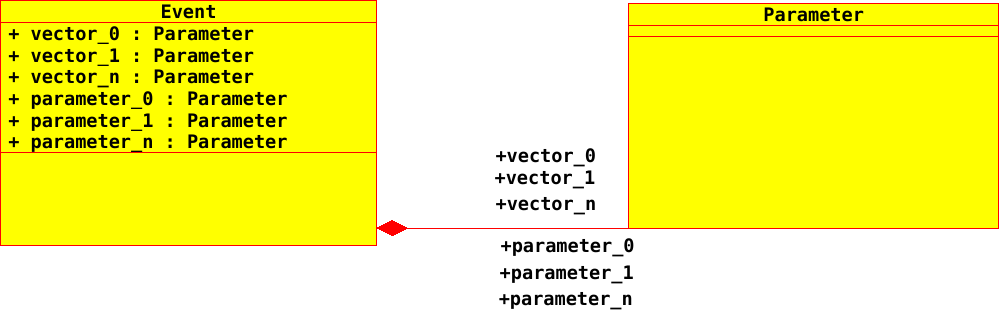
\includegraphics[scale=0.4]{uml_diagrams/event_parameter_basic_150.png}
% 
%     \caption{%
%         Ein Ereignis kann einen oder mehrere Vektoren enthalten.
%         Ein Ereignis kann einen oder mehrere Parameter enthalten.
%     }
% \end{figure}

\begin{table}[h!]
    \begin{center}
        \begin{tabular}{l l l l} 
            \hline
            Klassenname & ist Behälter & innere Verhältnisse & Beispiel \\ [0.5ex] 
            \hline\hline
            \texttt{SimpleEvent} & nein & - & ein Ton, ein Strich \\ 
            \texttt{SequentialEvent} & ja & akkumulierend & eine Melodie, ein Quadrat \\ 
            \texttt{SimultaneousEvent} & ja & parallel & Polyphonie, zwei Rechtecke \\ [1ex] 
            \hline
        \end{tabular}
    \end{center}

    \caption{Kernereignisse in \emph{mutwo}}
\end{table}

Ereignisse können andere Ereignisse enthalten oder keine anderen Ereignisse enthalten.
Falls Ereignisse andere Ereignisse enthalten, können die enthaltenen Ereignisse wiederrum iterativ weitere Ereignisse enthalten (Verschachtlung).
Falls ein Ereignis Ereignisse enthält, können diese entweder simultan (parallel) oder sequenziell (akkumulierend) angeordnet sein.
Mit den drei Ereignisklassen \texttt{SimpleEvent}, \texttt{SequentialEvent} und \texttt{SimultaneousEvent} sind alle Möglichkeiten darstellbar.

\begin{figure}[h!]
    \begin{center}
        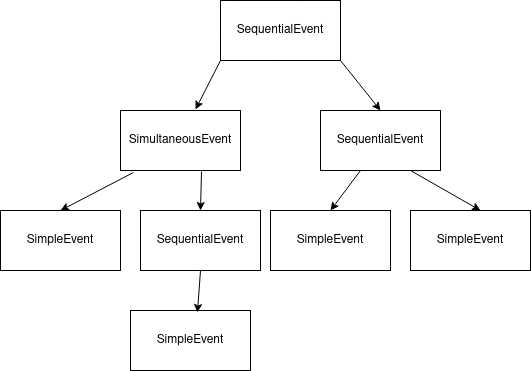
\includegraphics[scale=0.5]{pictures/nested_event.png}

        \caption{Exemplarische Verschachtlung von Ereignissen}
    \end{center}
\end{figure}


\subsubsection{Parameter}
\label{parameterSpecification}

Parameter repräsentieren generische Kategorien, die Ereignissen zugeordnet werden.
Generische Kategorien können beispielweise eine Farbe, eine Tonhöhe oder ein Luftdruck sein.

\bigskip

% XXX: Erwähne die abstrakte Klassen - Implementierungsdetails später (Entwicklungsstrategien)
% In \emph{mutwos} Design sind Parameter als abstrakte Klassen definiert, die eine minimale, öffentliche Programmierschnittstelle beschreiben.
% Diese minimale Schnittstelle versucht Parameter auf eine kompakte Identität zu reduzieren, die unabhängig ist von bestimmten Traditionen.
\emph{Mutwo} versucht Parameter über eine möglichst kompakte, generische Identität zu beschreiben.
Wenn möglich besteht diese kompakte Identität aus nur einem Wert (z. B. Zeichenkette oder Zahl).
Wenn möglich ist der Wert implizit einer physikalischen Einheit zugeordnet.

\begin{table}[h!]
    \begin{center}
        \begin{tabular}{l l} 
            \hline
            Parameter & Einheit \\ [0.5ex] 
            \hline\hline
            Tonhöhe & Hertz \\ 
            Tonhöhenintervall & Cents \\ 
            Dauer & beats \\ 
            Text & X-SAMPA\footnotemark \\ 
            Lautstärke & Volt \\ [1ex] 
            \hline
        \end{tabular}
    \end{center}

    \caption{Liste exemplarischer Ein-Wert-Parameter}
\end{table}

\footnotetext{%
    Das ``Extended Speech Assessment Methods Phonetic Alphabet'' ermöglicht die Darstellung der phonetischen IPA Symbole in ASCII.~\parencite{xsampaWikipedia}
}

\subsubsection{Übersetzer}

Ein Übersetzer transformiert eine Entität.
Entitäten sind entweder Objekte in Python oder externe Dateien.\footnote{%
    Objekte in Python können Instanzen von \emph{mutwo} internen Klassen, dritten Bibliotheken oder nativen Klassen sein.
    Externe Dateien umfassen beispielweise Mididateien oder Textdateien.
}
Transformieren bedeutet hier entweder eine Veränderung des Inhalts oder eine Veränderung des Formats.


\begin{table}[h!]
    % \hspace{-0.5cm}
    \begin{center}
        \smaller
        \begin{tabular}{l l l l} 
            \hline
            Klassenname & Eingangsentität & Ausgangsentität & Typ \\ [0.5ex] 
            \hline\hline
            \texttt{EventToMidiFile} & Instanz einer Ereignisklasse & Standard Midi File (SMF) & Format \\ 
            \texttt{MidiFileToEvent} & Standard Midi File (SMF) & Instanz einer Ereignisklasse & Format \\ 
            % XXX: Ist zu lange, kleinere Tabelle sieht schöner aus :)
            % \texttt{TwoPitchesToCommonHarmonicTuple} & Zwei Tonhöheninstanzen & Instanzen gemeinsamer Harmonischer & Inhalt \\ 
            \texttt{PitchToTabulaturaPitch} & Tonhöheninstanz & Tonhöheninstanz & Inhalt \\ [1ex] 
            \hline
        \end{tabular}

    \end{center}
    \caption{Exemplarische Übersetzer}
\end{table}

\smallskip


Übersetzer in \emph{mutwo} folgen einem funktionalem Paradigma, dh.\ ein Übersetzer verändert nicht die Eingangsentität (keine Seiteneffekte), sondern erzeugt eine neue, unabhängige Entität.
Das vereinfacht das Übersetzen derselben Entität mit unterschiedlichen Übersetzer.

\subsubsection{Generatoren}

Generatoren liefern (zumeist generische) Daten, die für generative Kunst nützlich sein mögen.
Generatoren umfassen Funktionen, Klassen, Konstanten oder andere Objekte.
Die Rückgabewerte der Funktionen und Klassen sind häufig Python native Objekte, die von Benutzern kreativ angewendet werden können.

\begin{table}[h!]
    \begin{center}
        \begin{tabular}{l l} 
            \hline
            Objekt & Beschreibung \\ [0.5ex] 
            \hline\hline
            \texttt{reflected\_binary\_code} & Erzeugt variable Gray-Codes \\
            \texttt{TUNEABLE\_INTERVAL\_TUPLE} & intonierbare Intervalle nach Marc Sabat \\
            \texttt{ActivityLevel} & Zyklen der Werte 0 und 1 nach Michael Edwards \\ [1ex] 
            \hline
        \end{tabular}
    \end{center}

    \caption{Exemplarische Generatoren}
\end{table}

%%%%%%%%%%%%%%%%%%%%%%%%%%%%%%%%%%%%%%%%%%%%%%%%%%%%%%%%%%%%%%%%%%%%%%%%%%%%%%%%%%%%%%%%%%%%
%%%%%%%%%%%%%%%%%%%%%%%%%%%%%%%%%%%%%%%%%%%%%%%%%%%%%%%%%%%%%%%%%%%%%%%%%%%%%%%%%%%%%%%%%%%%

\subsection{Entwicklungsstrategien}

\subsubsection{Programmiersprache}

\emph{Mutwo} ist in der Programmiersprache Python implementiert.
Python ist eine interpretierte, multi-paradigmatische, plattformübergreifende Sprache.
Sie wurde zum ersten Mal 1991 veröffentlicht.

\bigskip

Die Begründung für diese Wahl ist in den folgenden Punkten.

\begin{enumerate}
    \item{
            \textbf{Python ist einfach zu lernen und zu benutzen.}
            Pythons imperativer vereinfachter Syntax ist intuitiv rasch zu begreifen.
            Als interpretierte Sprache entfällt die Komplexität der Kompilierung.
            \emph{Mutwos} Zielgruppe sind nicht primär  professionelle Softwareentwickler:innen, sondern Künstler:innen.
            Deshalb ist eine flache, schnelle Lernkurve sehr bedeutend.
            % Das ist eine sehr wichtige Eigenschaft, weil \emph{mutwo} in erster Linie für und von  intendiert ist
    }
    \item{
            \textbf{Python ist populär.}
    }
    \item{
            \textbf{Python ist plattformübergreifend.}
    }
\end{enumerate}


\subsubsection{Strukturierung des Quellcodes}
\label{quellcodeStruktur}

Der Quellcode von \emph{mutwo} ist nach rigiden Regeln strukturiert.
Die Struktur basiert auf Pythons System von verschachtelten Modulen, Importe und Paketen.
Die Strenge der Struktur folgt zwei Absichten.
Erstens soll sie für Benutzer:innen einfach -- da konsistent und repetetiv -- verwendbar sein.
Zweitens vereinfacht sie die Entwicklung und Instandhaltung eines komplexen Softwareprojekts.

\bigskip

Der Paketname der Bibliothek ist \emph{mutwo}.
% XXX: Das ist ein unwichtiges Detail über Python, was nicht viel über mutwos Entwicklungsstrategien erzählt
% Pakete können im Python-Ökosystem auf der Plattform \emph{pypi} verwaltet werden.
% Mit dem standardisierten Pythonpaketmanager \emph{pip} können Pakete von \emph{pypi} installiert werden.
% 
% \lstset{language=bash}
% 
% \begin{lstlisting}
%     pip3 install mutwo
% \end{lstlisting}
% 
Das Paket \emph{mutwo} ist in unterschiedliche Module geteilt.
Die unterschiedlichen Module korrelieren mit den zuvor beschriebenen elementaren Bestandteilen von \emph{mutwo}.
Sie werden flankiert von zusätzlichen Hilfsmodulen.

\begin{table}[h!]
    \begin{center}
        \begin{tabular}{l l} 
            \hline
            Modulname & Modulbeschreibung \\ [0.5ex] 
            \hline\hline
            \texttt{configurations} & Globale modulübergreifende Konfigurationsvariablen \\
            \texttt{constants} & Globale modulübergreifende Konstanten \\
            \texttt{converters} & Import und Export von Daten, Übersetzen interner Strukturen \\
            \texttt{events} & Definition verschiedener Ereignisklassen \\
            \texttt{generators} & Generierung von für künstlerische Arbeiten hilfreiche Daten \\
            \texttt{parameters} & Klassen, deren Instanzen Ereignisattributen zugeordnet werden \\
            \texttt{version} & Versionsdefinition des Moduls \\
            \texttt{utilities} & Hilfsmethoden, Errordefinition \\ [1ex] 
            \hline
        \end{tabular}\label{table:modulDefinition}
    \end{center}

    \caption{Moduldefinitionen}
\end{table}

Module oder Pakete können in Python auf unterschiedliche Weisen importiert werden.
Die folgende Zeile dokumentiert die in \emph{mutwo} bevorzugte Weise:

\lstset{language=Python}

\begin{lstlisting}
    from mutwo import parameters
\end{lstlisting}

\emph{Mutwo} Module enthalten direkt die verwendbaren Objekte (Klassen, Funktionen).
Sie können nur eine limitierte Anzahl bestimmter Submodule enthalten.
Weil die Regel für alle \emph{mutwo} Module gilt ist sie einfach zu verstehen für neue Benutzer.
Sie korreliert mit der fünften Zeile des \emph{Zen of Python}:

\begin{quote}
    ``Flat is better than nested.''~\parencite{theZenOfPython}
\end{quote}

Folgende Tabelle beschreibt die möglichen Submodule eines Moduls:

\begin{table}[H]
    \begin{center}
        \begin{tabular}{l l} 
            \hline
            Submodulname & Modulbeschreibung \\ [0.5ex] 
            \hline\hline
            \texttt{abc} & Abstrakte Klassen \\  % Definition der gemeinsamen öffentlichen Schnittstelle (API)
            \texttt{configurations} & Globale modifizierbare Variablen zur Modulkonfiguration \\
            \texttt{constants} & Globale Konstanten des Moduls \\
            \hline
        \end{tabular}
    \end{center}

    \caption{Submoduldefinitionen}
\end{table}

Die Strukturierung des Quellcodes in thematisch getrennte Module und Submodule ist aber unzureichend.
Weil die grundsätzliche Designprämisse von sehr generischen Strukturen ausgeht, die aber präzise spezifiziert werden können, ist der potenzielle Umfang der Bibliothek schwer fasslich.
In \emph{mutwo} ist das Problem durch eine modulare Struktur von thematisch getrennten Paketen gelöst.
Jedes Paket hat einen einzigartigen Namen, hat eine unabhängige Version, kann eigene Abhängigkeiten definieren und ist je nach Abhängigkeitsstruktur unabhängig von anderen Paketen installierbar.

\bigskip

Die modulare Strukturierung in separate Pakete hilft nicht nur der Entwicklung und Instandhaltung, sondern ermöglicht auch Nutzern nur diejenigen Programmbestandteile zu installieren, die für ein bestimmtes Projekt benötigt werden.
Das macht die Bibliothek leichter.
Mit der modularen Struktur können Dritte unkompliziert die Bibliothek durch weitere Funktionen erweitern.
Sie können einfach ein neues Paket dem \emph{mutwo} Ökosystem hinzufügen.

\bigskip

Technisch ist die Modularität durch Pythons Unterstützung von \emph{namespace packages} gelöst.
Das ermöglicht voneinander unabhängigen Pakete die Installation von Quellcode unter einem gemeinsamen Paketnamen.

\bigskip

Einzelne Pakete im \emph{mutwo} Ökosystem sind auf standardisierte Weise benannt.
Ihr Name setzt sich durch das Wort \emph{mutwo} und einem Begriff für die enthaltenen Funktionen zusammen.

\bigskip

\hspace{0.5cm}
\begin{minipage}{0.95\textwidth}
    \begin{description}[style=multiline, leftmargin=3.25cm, font=\normalfont\emph]
        \item[mutwo.core] Kunstform-, medien- und kulturagnostische Objekte
        \item[mutwo.music] Musikspezifische Objekte
        \item[mutwo.reaper] Funktionen, die mit der DAW Reaper zusammenhängen
    \end{description}
\end{minipage}

\bigskip

Das \emph{mutwo} Ökosystem setzt die anfänglich beschriebene Struktur von Modulen und Submodulen auch in separaten Paketen um.
Die Namen der Module sind Kompositionen aus einem Präfix und einem Suffix.
Der Präfix ist der Suffix des Paketnamen (z. B. \texttt{core} oder \texttt{music}).
Der Suffix beschreibt die Funktion des Moduls (z. B. \texttt{events} oder \texttt{parameters}).
Präfix und Suffix sind durch einen Unterstrich getrennt.

\begin{table}[H]
    \begin{center}
        \begin{tabular}{l l l}
            \hline
            Paketidentität (Präfix) & Modulfunktion (Suffix) & Modulname \\ [0.5ex] 
            \hline\hline
            \texttt{core} & \texttt{parameters} & \texttt{core\_parameters} \\
            \texttt{music} & \texttt{events} & \texttt{music\_events} \\
            \texttt{midi} & \texttt{converters} & \texttt{midi\_converters} \\
            \hline
        \end{tabular}
    \end{center}

    \caption{Exemplarische Module}
\end{table}

Das Importieren im Quellcode funktioniert auf gleiche Weise wie oben beschrieben:

\begin{lstlisting}
    from mutwo import core_parameters
    from mutwo import music_events
    from mutwo import midi_converters
\end{lstlisting}

\subsubsection{Abstrakte Basisklassen}

Wie in \emph{\nameref{quellcodeStruktur}} vorgestellt, enthält jedes \emph{mutwo} Modul potenziell das \texttt{abc}~\footnote{%
    i.\ e. \emph{abstract base classes}%
} Teilmodul.
In diesen Modul werden abstrakte Klassen definiert.
Abstrakte Klassen sind Klassen deren Methoden oder Attribute nicht oder nur stellenweise implementiert sind.
Abstrakte Klassen können deshalb nicht initialisiert werden.
Von abstrakten Klassen können unterschiedliche dritte Klassen erben, die fehlende Teile implementieren.
Sind alle fehlende Teile implementiert, kann eine abgeleitete Klasse initialisiert werden~\parencite{abstractTypeWiki}.

\bigskip

In \emph{mutwo} ermöglichen abstrakte Klassen die Definition der öffentlichen Schnittstelle (API) einer Programmkomponente.
Verschiedene, zusammenhängende Programmkomponente erwarten voneinander entsprechende API.
Sie sind damit unabhängig von spezifischen Implementierungen.
Diese Technologie unterliegt der im im Kapitel \emph{\nameref{parameterSpecification}} beschriebene Definition der Parameterklassen.
Die im \texttt{abc} Teilmodul des \texttt{parameters} Modul deklarierte Klassen definieren so ihre kompakte Identität über ein nicht--implementiertes Attribut.

\begin{table}[h!]
    \begin{center}
        \begin{tabular}{l l l l} 
            \hline
            Parameter & Klassenname & Abstraktes Attribut & Attributdatentyp \\ [0.5ex] 
            \hline\hline
            Tonhöhe & \texttt{Pitch} & \texttt{frequency} & Gleitkommazahl \\ 
            Tonhöhenintervall & \texttt{PitchInterval} & \texttt{interval} & Gleitkommazahl \\ 
            Dauer & \texttt{Duration} & \texttt{duration} & Bruch \\ 
            Text & \texttt{Lyric} & \texttt{phonetic\_script} & Zeichenkette \\ 
            Lautstärke & \texttt{Volume} & \texttt{amplitude} & Gleitkommazahl \\ [1ex] 
            \hline
        \end{tabular}
    \end{center}

    \caption{Präzision der Liste exemplarischer Ein-Wert-Parameter}
\end{table}

Dritte Bestandteile \emph{mutwos} erwarten nur diese minimal--definierte Schnittstelle.
Das ermöglicht Benutzern die Implementierung einer Repräsentation einer Kategorie, die der jeweiligen Interpretation entspricht.
Das Design \emph{mutwos} versichert, dass die von Benutzern hinzugefügten Repräsentationen mit anderen Bibliothekskomponenten kompatibel sind.

\begin{figure}[h!]
    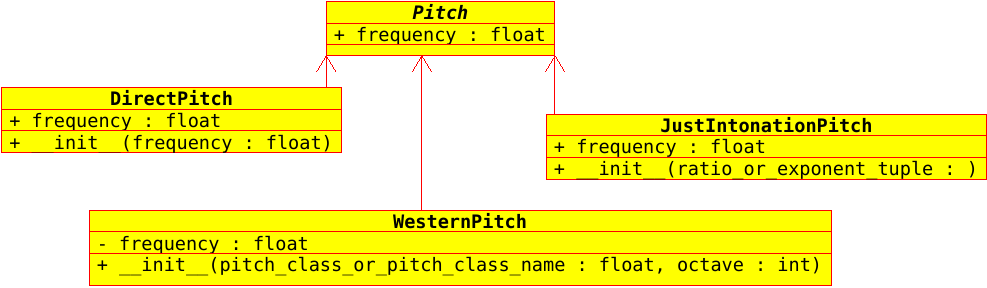
\includegraphics[scale=0.4]{uml_diagrams/pitches.png}

    \caption{%
        Schematische Darstellung eines Parameter und seine unterschiedliche Subklassen.
        Die Subklassen ermöglichen unterschiedliche Perspektiven derselben Entität.
        Sie werden mit unterschiedlichen Argumenten initialisiert.
    }

\end{figure}

\subsubsection{\emph{Konvention vor Konfiguration} (Sensible Voreinstellungen)}

Das Entwicklungsparadigma \emph{Konvention vor Konfiguration} entspannt den in \emph{\nameref{motivationUndAbsicht}} beschriebenen Konflikt zwischen Anpassbarkeit und Einfachheit.
Viele Funktionen und Methoden \emph{mutwos} haben eine große Anzahl potenzieller Argumente.
Häufig ist Intention der reichen Argumente das generische, adaptive Designziel zu erfüllen.
Benutzer:innen werden für einige Argumente selten eine Notwendigkeit entwickeln, diese explizit zu deklarieren.

\bigskip

In dieser Situation kann genanntes Paradigma helfen.
\emph{Konvention vor Konfiguration} empfiehlt, dass Benutzer:innen einer Bibliothek nur unkonventionelle Konfigurationen spezifizieren müssen~\parencite{conventionOverConfiguration}.

\bigskip

\emph{Mutwo} realisiert diese Empfehlung mithilfe sensibler Voreinstellungen.
Viele Argumente haben voreingestellte Standardwerte.
Wird kein expliziter Wert deklariert, fallen Funktionen und Methoden auf diese zurück.
Dadurch müssen Benutzer:innen nur elementare oder für sie relevante Argumente angeben.

\bigskip

Dieses Paradigma birgt die Gefahr bestimmte (Musik--)Traditionen oder Ästhetiken zu priorisieren.
Die Gefahr ist darin begründet, dass manche (die den Konventionen entsprechenden) Lösungen einfacher umzusetzen sind als andere.
In meinem Verständnis wiegt der Mehrwert einer einfachen, intuitiven und von Standardformulierungen befreiten Anwendung diese Gefahr auf.

\subsubsection{Globale Voreinstellungen}

Um beschriebene Gefahr weiter einzudämmen vereinfacht \emph{mutwo} das Überschreiben der Voreinstellungen mithilfe globaler Variablen.
Wird kein expliziter Wert deklariert, weisen Funktionen und Methoden während der Laufzeit dynamisch die Werte ihrer Argumente diesen Variablen zu.

\begin{center}
    \fbox{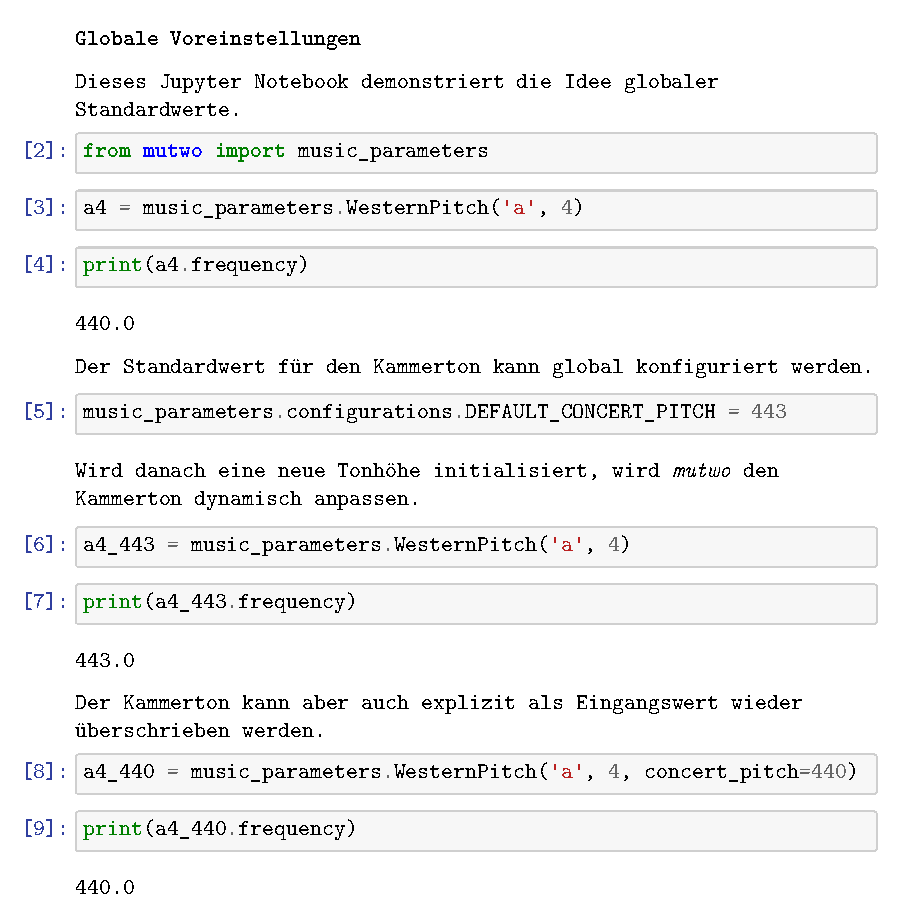
\includegraphics[page=1,scale=0.95]{jupyter/Globale_Voreinstellungen.pdf}}
\end{center}

\subsubsection{Dokumentation öffentlicher Schnittstellen}

\subsubsection{Funktionen als Argumente}

\subsubsection{Dynamische Zuweisung von Attributen}

\subsubsection{Trennung von format-, programm-, protokollspezifischen Darstellungen und interner Repräsentation}

\subsubsection{Abwesenheit vorgegebener Arbeitsmodelle}

\subsubsection{Deskriptive Fehlermeldungen und Warnungen}

\subsubsection{Warnungen statt Fehler}

\subsubsection{Annotation von Typen im Quellcode}

\subsubsection{Rigide Namenskonventionen}


%%%%%%%%%%%%%%%%%%%%%%%%%%%%%%%%%%%%%%%%%%%%%%%%%%%%%%%%%%%%%%%%%%%%%%%%%%%%%%%%%%%%%%%%%%%%
%%%%%%%%%%%%%%%%%%%%%%%%%%%%%%%%%%%%%%%%%%%%%%%%%%%%%%%%%%%%%%%%%%%%%%%%%%%%%%%%%%%%%%%%%%%%

\subsection{Limitierungen und Grenzen}


%%%%%%%%%%%%%%%%%%%%%%%%%%%%%%%%%%%%%%%%%%%%%%%%%%%%%%%%%%%%%%%%%%%%%%%%%%%%%%%%%%%%%%%%%%%%
%%%%%%%%%%%%%%%%%%%%%%%%%%%%%%%%%%%%%%%%%%%%%%%%%%%%%%%%%%%%%%%%%%%%%%%%%%%%%%%%%%%%%%%%%%%%

\subsection{Beispiel-orientierte Einführung}

%%%%%%%%%%%%%%%%%%%%%%%%%%%%%%%%%%%%%%%%%%%%%%%%%%%%%%%%%%%%%%%%%%%%%%%%%%%%%%%%%%%%%%%%%%%%
%%%%%%%%%%%%%%%%%%%%%%%%%%%%%%%%%%%%%%%%%%%%%%%%%%%%%%%%%%%%%%%%%%%%%%%%%%%%%%%%%%%%%%%%%%%%

\subsection{Fallstudien}

\subsubsection{\emph{thanatos trees for Tim Pauli}}

\subsubsection{\emph{ohne Titel (2)} und \emph{ohne Titel (3)}}

\section{Zusammenfassung}

\subsection{Richtungen weiterer Entwicklungen}

\subsection{Evaluation}

\newpage

\appendix

\printbibliography

\newpage

\listoffigures

\newpage


\end{document}
